\documentclass[11pt]{report}

\usepackage{hyperref}

\usepackage[french]{babel}
\usepackage[utf8]{inputenc}
\usepackage[T1]{fontenc}

\usepackage{amsmath}  % Maths
\usepackage{amsfonts} % Maths
\usepackage{amssymb}  % Maths
\usepackage{stmaryrd} % Maths (crochets doubles)

\usepackage{url}     % Mise en forme + liens pour URLs
\usepackage{array}   % Tableaux évolués

\usepackage{algorithm}
\usepackage{algorithmic}
\usepackage{comment}

\usepackage[hmargin=3cm,vmargin=2.5cm]{geometry}

\usepackage{tikz}
\newdimen\pgfex
\newdimen\pgfem
\usetikzlibrary{arrows,shapes,shadows,scopes}
\usetikzlibrary{positioning}
\usetikzlibrary{matrix}
\usetikzlibrary{decorations.text}
\usetikzlibrary{decorations.pathmorphing}






%%%%%%%%%%%%%%%%%%%%%%%%%%%%%%%%%%%%%%%%%%%%%%%%%%%%%%%%%%%%%%%%%%%%%%%%%%%%%%%%%%%%%%%%%%%
%%%%%%%%%%%%%%%%%%%%%%%%%%%%%%%%%%%%%%%%%%%%%%%%%%%%%%%%%%%%%%%%%%%%%%%%%%%%%%%%%%%%%%%%%%%
%%%%%%%%%%%%%%%%%%Definition des éléments pour un reseau de signalisation%%%%%%%%%%%%%%%%%
\definecolor{pinegreen}{cmyk}{0.92,0,0.59,0.25}
\definecolor{royalblue}{cmyk}{1,0.50,0,0}
\definecolor{lavander}{cmyk}{0,0.48,0,0}
\definecolor{violet}{cmyk}{0.79,0.88,0,0}
\tikzstyle{sn}=[circle, draw, thin,fill=cyan!20, scale=0.8] %seed node
\tikzstyle{ps}=[rectangle, draw, thin,fill=green!20, scale=0.8] %protein de signalisation
\tikzstyle{cplx}=[square, draw, thin, fill=white!20, scale=0.7] %définition d'un complex
\tikzstyle{transl}=[diamond, draw, thin, fill=white!20, scale=0.3]
\tikzstyle{mod}=[triangle, draw, thin, fill=white!20, scale=0.3]
\tikzstyle{qgre}=[rectangle, draw, thin,fill=green!20, size=15pts]
\tikzstyle{tgrn}=[triangle, draw, thin, fill=green!20, scale=0.8]

%Ajout des arc qui ne sont pas définis dans le grn
\tikzstyle{st}=[->, draw, thin, dashed] %définition d'un state transition


% Macros relatives à la traduction de PH avec arcs neutralisants vers PH à k-priorités fixes

% Macros générales
\def\Pint{\textsc{PINT}}

% Notations générales pour PH
\newcommand{\PH}{\mathcal{PH}}
\newcommand{\PHs}{\Sigma}
\newcommand{\PHl}{L}
%\newcommand{\PHp}{\mathcal{P}}
\newcommand{\PHp}{\textcolor{red}{\mathcal{P}}}
\newcommand{\PHproc}{\mathcal{P}}
\newcommand{\PHa}{\PHh}
\newcommand{\PHh}{\mathcal{H}}
\newcommand{\PHn}{\mathcal{N}}

\newcommand{\PHhitter}{\mathsf{hitter}}
\newcommand{\PHtarget}{\mathsf{target}}
\newcommand{\PHbounce}{\mathsf{bounce}}
\newcommand{\PHsort}{\Sigma}

\def\f#1{\mathsf{#1}}
\def\focals{\f{focals}}
\def\play{\cdot}
\def\configs#1{\mathbb C_{#1\rightarrow a}}

%\newcommand{\PHfrappeR}{\textcolor{red}{\rightarrow}}
%\newcommand{\PHmonte}{\textcolor{red}{\Rsh}}

\newcommand{\PHfrappeA}{\rightarrow}
\newcommand{\PHfrappeB}{\Rsh}
%\newcommand{\PHfrappe}[3]{\mbox{$#1\PHfrappeA#2\PHfrappeB#3$}}
%\newcommand{\PHfrappebond}[2]{\mbox{$#1\PHfrappeB#2$}}
\newcommand{\PHfrappe}[3]{#1\PHfrappeA#2\PHfrappeB#3}
\newcommand{\PHfrappebond}[2]{#1\PHfrappeB#2}
\newcommand{\PHobjectif}[2]{\mbox{$#1\PHfrappeB^*\!#2$}}
\newcommand{\PHconcat}{::}
\newcommand{\PHneutralise}{\rtimes}

\def\PHget#1#2{{#1[#2]}}
%\newcommand{\PHchange}[2]{#1\langle #2 \rangle}
\newcommand{\PHchange}[2]{(#1 \Lleftarrow #2)}
\newcommand{\PHarcn}[2]{\mbox{$#1\PHneutralise#2$}}
\newcommand{\PHjoue}{\cdot}

\newcommand{\PHetat}[1]{\mbox{$\langle #1 \rangle$}}


% Notations spécifiques à ce papier
\newcommand{\PHdirectpredec}[1]{\PHs^{-1}(#1)}
\newcommand{\PHpredec}[1]{\f{pred}(#1)}
\newcommand{\PHpredecgene}[1]{\f{reg}({#1})}
\newcommand{\PHpredeccs}[1]{\PHpredec{#1} \setminus \Gamma}

\newcommand{\PHincl}[2]{#1 :: #2}

\def\ctx{\varsigma}
\def\ctxOverride{\Cap}
\def\state#1{\langle #1 \rangle}

% Notations spécifiques aux graphes d'états
%\newcommand{\PHge}{\textcolor{red}{\mathcal{GE}}}
%\newcommand{\PHt}{\mathcal{T}}
%\newcommand{\GE}{\mathcal{GE}}
%\newcommand{\GEt}{\mathcal{T}}
%\newcommand{\GEl}{\PHl}
%\newcommand{\GEa}{\PHa}
%\newcommand{\GEva}[3]{#1 \stackrel{#2}{\longrightarrow} #3}
%\newcommand{\GEval}[3]{#1 \stackrel{#2}{\Longrightarrow} #3}
%\newcommand{\GEget}[2]{\PHget{#1}{#2}}


\def\DEF{\stackrel{\Delta}=}
\def\EQDEF{\stackrel{\Delta}\Leftrightarrow}

\def\intervalless{<_{[]}}


\usepackage{ifthen}
\usepackage{tikz}
\usetikzlibrary{arrows,shapes}

\definecolor{lightgray}{rgb}{0.8,0.8,0.8}
\definecolor{lightgrey}{rgb}{0.8,0.8,0.8}

\tikzstyle{boxed ph}=[]
\tikzstyle{sort}=[fill=lightgray,rounded corners]
\tikzstyle{process}=[circle,draw,minimum size=15pt,fill=white,
font=\footnotesize,inner sep=1pt]
\tikzstyle{black process}=[process, fill=black,text=white, font=\bfseries]
\tikzstyle{gray process}=[process, draw=black, fill=lightgray]
\tikzstyle{current process}=[process, draw=black, fill=lightgray]
\tikzstyle{process box}=[white,draw=black,rounded corners]
\tikzstyle{tick label}=[font=\footnotesize]
\tikzstyle{tick}=[black,-]%,densely dotted]
\tikzstyle{hit}=[->,>=angle 45]
\tikzstyle{selfhit}=[min distance=30pt,curve to]
\tikzstyle{bounce}=[densely dotted,->,>=latex]
\tikzstyle{hl}=[font=\bfseries,very thick]
\tikzstyle{hl2}=[hl]
\tikzstyle{nohl}=[font=\normalfont,thin]

\newcommand{\currentScope}{}
\newcommand{\currentSort}{}
\newcommand{\currentSortLabel}{}
\newcommand{\currentAlign}{}
\newcommand{\currentSize}{}

\newcounter{la}
\newcommand{\TSetSortLabel}[2]{
  \expandafter\repcommand\expandafter{\csname TUserSort@#1\endcsname}{#2}
}
\newcommand{\TSort}[4]{
  \renewcommand{\currentScope}{#1}
  \renewcommand{\currentSort}{#2}
  \renewcommand{\currentSize}{#3}
  \renewcommand{\currentAlign}{#4}
  \ifcsname TUserSort@\currentSort\endcsname
    \renewcommand{\currentSortLabel}{\csname TUserSort@\currentSort\endcsname}
  \else
    \renewcommand{\currentSortLabel}{\currentSort}
  \fi
  \begin{scope}[shift={\currentScope}]
  \ifthenelse{\equal{\currentAlign}{l}}{
    \filldraw[process box] (-0.5,-0.5) rectangle (0.5,\currentSize-0.5);
    \node[sort] at (-0.2,\currentSize-0.4) {\currentSortLabel};
   }{\ifthenelse{\equal{\currentAlign}{r}}{
     \filldraw[process box] (-0.5,-0.5) rectangle (0.5,\currentSize-0.5);
     \node[sort] at (0.2,\currentSize-0.4) {\currentSortLabel};
   }{
    \filldraw[process box] (-0.5,-0.5) rectangle (\currentSize-0.5,0.5);
    \ifthenelse{\equal{\currentAlign}{t}}{
      \node[sort,anchor=east] at (-0.3,0.2) {\currentSortLabel};
    }{
      \node[sort] at (-0.6,-0.2) {\currentSortLabel};
    }
   }}
  \setcounter{la}{\currentSize}
  \addtocounter{la}{-1}
  \foreach \i in {0,...,\value{la}} {
    \TProc{\i}
  }
  \end{scope}
}

\newcommand{\TTickProc}[2]{ % pos, label
  \ifthenelse{\equal{\currentAlign}{l}}{
    \draw[tick] (-0.6,#1) -- (-0.4,#1);
    \node[tick label, anchor=east] at (-0.55,#1) {#2};
   }{\ifthenelse{\equal{\currentAlign}{r}}{
    \draw[tick] (0.6,#1) -- (0.4,#1);
    \node[tick label, anchor=west] at (0.55,#1) {#2};
   }{
    \ifthenelse{\equal{\currentAlign}{t}}{
      \draw[tick] (#1,0.6) -- (#1,0.4);
      \node[tick label, anchor=south] at (#1,0.55) {#2};
    }{
      \draw[tick] (#1,-0.6) -- (#1,-0.4);
      \node[tick label, anchor=north] at (#1,-0.55) {#2};
    }
   }}
}
\newcommand{\TSetTick}[3]{
  \expandafter\repcommand\expandafter{\csname TUserTick@#1_#2\endcsname}{#3}
}

\newcommand{\myProc}[3]{
  \ifcsname TUserTick@\currentSort_#1\endcsname
    \TTickProc{#1}{\csname TUserTick@\currentSort_#1\endcsname}
  \else
    \TTickProc{#1}{#1}
  \fi
  \ifthenelse{\equal{\currentAlign}{l}\or\equal{\currentAlign}{r}}{
    \node[#2] (\currentSort_#1) at (0,#1) {#3};
  }{
    \node[#2] (\currentSort_#1) at (#1,0) {#3};
  }
}
\newcommand{\TSetProcStyle}[2]{
  \expandafter\repcommand\expandafter{\csname TUserProcStyle@#1\endcsname}{#2}
}
\newcommand{\TProc}[1]{
  \ifcsname TUserProcStyle@\currentSort_#1\endcsname
    \myProc{#1}{\csname TUserProcStyle@\currentSort_#1\endcsname}{}
  \else
    \myProc{#1}{process}{}
  \fi
}

\newcommand{\repcommand}[2]{
  \providecommand{#1}{#2}
  \renewcommand{#1}{#2}
}
\newcommand{\THit}[5]{
  \path[hit] (#1) edge[#2] (#3#4);
  \expandafter\repcommand\expandafter{\csname TBounce@#3@#5\endcsname}{#4}
}
\newcommand{\TBounce}[4]{
  (#1\csname TBounce@#1@#3\endcsname) edge[#2] (#3#4)
}

\newcommand{\TState}[1]{
  \foreach \proc in {#1} {
    \node[current process] (\proc) at (\proc.center) {};
  }
}

% Macros spécifiques au Modèle de Thomas / aux RRB

% Notations pour le modèle de Thomas (depuis thèse)
\newcommand{\GRN}{\mathcal{GRN}}
\newcommand{\IG}{\mathcal{G}}
%\def\IG{\mathrm{IG}}
\newcommand{\GRNreg}[1]{\Gamma^{-1}(#1)}
\newcommand{\GRNres}[2]{\mathsf{Res}_{#1}(#2)}
\newcommand{\GRNallres}[1]{\mathsf{Res}_{#1}}
\newcommand{\GRNget}[2]{\PHget{#1}{#2}}
\newcommand{\GRNetat}[1]{\PHetat{#1}}

\def\levels{\mathsf{levels}}
\def\levelsA#1#2{\levels_+(#1\rightarrow #2)}
\def\levelsI#1#2{\levels_-(#1\rightarrow #2)}
%\newcommand{\PHres}{\mathsf{Res}}

\newcommand{\Kinconnu}{\emptyset}
\newcommand{\RRGva}[3]{#1 \stackrel{#2}{\longrightarrow} #3}
\newcommand{\RRGgi}{\mathcal{G}}
\newcommand{\RRGreg}[1]{\RRGgi_{#1}}



%\definecolor{darkred}{rgb}{0.5,0,0}
%\definecolor{lightred}{rgb}{1,0.8,0.8}
%\definecolor{lightgreen}{rgb}{0.7,1,0.7}
\definecolor{darkgreen}{rgb}{0,0.5,0}
%\definecolor{darkyellow}{rgb}{0.5,0.5,0}
%\definecolor{lightyellow}{rgb}{1,1,0.6}
%\definecolor{darkcyan}{rgb}{0,0.6,0.6}
%\definecolor{darkorange}{rgb}{0.8,0.2,0}

%\definecolor{notsodarkgreen}{rgb}{0,0.7,0}

%\definecolor{coloract}{rgb}{0,1,0}
%\definecolor{colorinh}{rgb}{1,0,0}
\colorlet{coloract}{darkgreen}
\colorlet{colorinh}{red}
%\colorlet{coloractgray}{lightgreen}
%\colorlet{colorinhgray}{lightred}
%\colorlet{colorinf}{darkgray}
%\colorlet{coloractgray}{lightgreen}
%\colorlet{colorinhgray}{lightred}

%\colorlet{colorgray}{lightgray}


\tikzstyle{grn}=[every node/.style={circle,draw=black,outer sep=2pt,minimum
                size=15pt,text=black}, node distance=1.5cm]
\tikzstyle{act}=[->,draw=black,thick,color=black]
\tikzstyle{inh}=[>=|,-|,draw=black,thick, text=black,label]
%\tikzstyle{inh}=[>=|,-|,draw=colorinh,thick, text=black,label]
%\tikzstyle{act}=[->,>=triangle 60,draw=coloract,thick,color=coloract]
%\tikzstyle{inhgray}=[>=|,-|,draw=colorinhgray,thick, text=black,label]
%\tikzstyle{actgray}=[->,>=triangle 60,draw=coloractgray,thick,color=coloractgray]
\tikzstyle{inf}=[->,draw=colorinf,thick,color=colorinf]
%\tikzstyle{elabel}=[fill=none, above=-1pt, sloped,text=black, minimum size=10pt, outer sep=0, font=\scriptsize,draw=none]
\tikzstyle{elabel}=[fill=none,text=black, above=-2pt,%sloped,
minimum size=10pt, outer sep=0, font=\scriptsize, draw=none]
%\tikzstyle{elabel}=[]
\tikzstyle{sg}=[every node/.style={outer sep=2pt,minimum
                size=15pt,text=black}, node distance=2cm]



% Commandes À FAIRE
\usepackage{color} % Couleurs du texte
\definecolor{darkgreen}{rgb}{0,0.5,0}
%\newcommand{\afaire}[1]{\textcolor{red}{[À FAIRE~: #1]}}
%\newcommand{\resume}[1]{\textcolor{blue}{#1}}
\newcommand{\todo}[1]{\textcolor{darkgreen}{[#1]}}
\newcolumntype{M}[1]{>{\raggedright}m{#1}}


% Id est
\newcommand{\ie}{\textit{i.e.} }



\title{Rapport pour le comité de suivi de thèse 2013/2014}

\author{Louis Fippo Fitime}

%LUNAM Universit\'e, \'Ecole Centrale de Nantes, IRCCyN UMR CNRS 6597\\
%(Institut de Recherche en Communications et Cybern\'etique de Nantes)\\
%1 rue de la No\"e -- B.P. 92101 -- 44321 Nantes Cedex 3, France.\\
%\email{Louis.Fippo-Fitime@irccyn.ec-nantes.fr}

\begin{document}

%\maketitle

% Exemples

%%% Exemple pour la définition du Process Hitting %%%
\def \exphdef {
\path[use as bounding box] (-0.5,-0.5) rectangle (6.5,4.5);

\TSort{(0,3)}{a}{2}{l}
\TSort{(0,0)}{b}{2}{l}
\TSort{(6,1)}{z}{3}{r}

\THit{a_1}{}{z_1}{.west}{z_2}
\THit{b_1}{}{z_0}{.west}{z_1}
\THit{a_0}{out=250,in=200,selfhit}{a_0}{.west}{a_1}

\path[bounce,bend left]
\TBounce{z_0}{}{z_1}{.south}
\TBounce{z_1}{}{z_2}{.south}
\TBounce{a_0}{}{a_1}{.south}
;
}



%%% Exemple pour la coopération %%%
\def \exphcoop {
\path[use as bounding box] (-0.5,-0.5) rectangle (6.5,4.5);

% Actions de màj grisées
\only<6->{
\THit{a_1}{ulhit,color=lightgray}{ab_0}{.west}{ab_2}
\THit{a_1}{ulhit,color=lightgray}{ab_1}{.west}{ab_3}
\path[bounce,bend left,pulhit] \TBounce{ab_0}{bulhit}{ab_2}{.south} \TBounce{ab_1}{bulhit}{ab_3}{.south} ;
}

\only<7->{
\THit{a_0}{ulhit}{ab_2}{.west}{ab_0}
\THit{a_0}{ulhit}{ab_3}{.west}{ab_1}
\path[bounce,bend right,pulhit] \TBounce{ab_2}{bulhit}{ab_0}{.north} \TBounce{ab_3}{bulhit}{ab_1}{.north} ;
}

\only<8->{
\THit{b_0}{ulhit}{ab_3}{.west}{ab_2}
\THit{b_0}{ulhit}{ab_1}{.west}{ab_0}
\THit{b_1}{ulhit}{ab_0}{.west}{ab_1}
\THit{b_1}{ulhit}{ab_2}{.west}{ab_3}
\path[bounce,bend right,pulhit] \TBounce{ab_1}{bulhit}{ab_0}{.north} \TBounce{ab_3}{bulhit}{ab_2}{.north} ;
\path[bounce,bend left,pulhit] \TBounce{ab_0}{bulhit}{ab_1}{.south} \TBounce{ab_2}{bulhit}{ab_3}{.south} ;
}

% Sortes
\TSort{(0,3)}{a}{2}{l}
\TSort{(0,0)}{b}{2}{l}
\TSort{(6,1)}{z}{3}{r}

% Deux actions disjointes en exemple
\only<2-3>{
\THit{a_1}{}{z_1}{.north west}{z_2}
\path[bounce,bend left]
\TBounce{z_1}{}{z_2}{.south} ;

\THit{b_0}{}{z_1}{.west}{z_2}
\path[bounce,bend left=55]
\TBounce{z_1}{}{z_2}{.south west} ;
}

% Processus d'exemple
\TState{3}{a_1,b_1,z_1}

% Sorte coopérative et arcs
\only<4->{
\TSetTick{ab}{0}{00}
\TSetTick{ab}{1}{01}
\TSetTick{ab}{2}{10}
\TSetTick{ab}{3}{11}
\TSort{(3,0.5)}{ab}{4}{l}
}

% Arcs de màj noirs de la sc
\only<5>{
\THit{a_1}{thick}{ab_0}{.west}{ab_2}
\THit{a_1}{thick}{ab_1}{.west}{ab_3}
\path[bounce,thick,bend left] \TBounce{ab_0}{thick}{ab_2}{.south} \TBounce{ab_1}{thick}{ab_3}{.south} ;
}

\only<6>{
\THit{a_0}{thick}{ab_2}{.west}{ab_0}
\THit{a_0}{thick}{ab_3}{.west}{ab_1}
\path[bounce,thick,bend right] \TBounce{ab_2}{thick}{ab_0}{.north} \TBounce{ab_3}{thick}{ab_1}{.north} ;
}

\only<7>{
\THit{b_0}{thick}{ab_3}{.west}{ab_2}
\THit{b_0}{thick}{ab_1}{.west}{ab_0}
\THit{b_1}{thick}{ab_0}{.west}{ab_1}
\THit{b_1}{thick}{ab_2}{.west}{ab_3}
\path[bounce,thick,bend right] \TBounce{ab_1}{thick}{ab_0}{.north} \TBounce{ab_3}{thick}{ab_2}{.north} ;
\path[bounce,thick,bend left] \TBounce{ab_0}{thick}{ab_1}{.south} \TBounce{ab_2}{thick}{ab_3}{.south} ;
}

% État d'exemple pour màj de la sc
\TState{8-9}{a_1,b_0}
\TState{10}{a_1,b_0,ab_0,ab_1,ab_2,ab_3}
\TState{11}{a_1,b_0,ab_2}
\only<9-11>{
\THit{a_1}{}{ab_0}{.west}{ab_2}
\THit{a_1}{}{ab_1}{.west}{ab_3}
\THit{b_0}{}{ab_3}{.west}{ab_2}
\THit{b_0}{}{ab_1}{.west}{ab_0}
\path[bounce,bend left] \TBounce{ab_0}{}{ab_2}{.south} \TBounce{ab_1}{}{ab_3}{.south} ;
\path[bounce,bend right] \TBounce{ab_1}{}{ab_0}{.north} \TBounce{ab_3}{}{ab_2}{.north} ;
}

% État d'exemple pour action de la sc
\TState{12}{a_1,b_0,z_1,ab_2}
\TState{13-14}{a_1,b_0,z_2,ab_2}

% Arc sortant de la sc
\only<12-14>{
\THit{ab_2}{thick}{z_1}{.west}{z_2}
\path[bounce,bend left,thick] \TBounce{z_1}{thick}{z_2}{.south} ;
}

% Arc sortant de la sc
\only<15->{
\THit{ab_2}{}{z_1}{.west}{z_2}
\path[bounce,bend left] \TBounce{z_1}{}{z_2}{.south} ;
}

}



%%% Exemple pour l'inférence %%%
\def \exphinf {
% Sortes
\TSort{(0,3)}{a}{2}{l}
\TSort{(0,0)}{b}{2}{l}
\TSort{(6,0)}{z}{3}{r}

% Sorte coopérative et arcs
\TSetTick{ab}{0}{00}
\TSetTick{ab}{1}{01}
\TSetTick{ab}{2}{10}
\TSetTick{ab}{3}{11}
\TSort{(3,0)}{ab}{4}{l}

% Actions de màj grisées
\THit{a_1}{ulhit}{ab_0}{.west}{ab_2}
\THit{a_1}{ulhit}{ab_1}{.west}{ab_3}
\path[bounce,bend left,pulhit] \TBounce{ab_0}{bulhit}{ab_2}{.south} \TBounce{ab_1}{bulhit}{ab_3}{.south};

\THit{a_0}{ulhit}{ab_2}{.west}{ab_0}
\THit{a_0}{ulhit}{ab_3}{.west}{ab_1}
\path[bounce,bend right,pulhit] \TBounce{ab_2}{bulhit}{ab_0}{.north} \TBounce{ab_3}{bulhit}{ab_1}{.north};

\THit{b_0}{ulhit}{ab_3}{.west}{ab_2}
\THit{b_0}{ulhit}{ab_1}{.west}{ab_0}
\THit{b_1}{ulhit}{ab_0}{.west}{ab_1}
\THit{b_1}{ulhit}{ab_2}{.west}{ab_3}
\path[bounce,bend right,pulhit] \TBounce{ab_1}{bulhit}{ab_0}{.north} \TBounce{ab_3}{bulhit}{ab_2}{.north};
\path[bounce,bend left,pulhit] \TBounce{ab_0}{bulhit}{ab_1}{.south} \TBounce{ab_2}{bulhit}{ab_3}{.south};

% Arcs sortant de la sc
\THit{ab_2}{ulhit}{z_1}{.north west}{z_2}
\THit{ab_2}{ulhit}{z_0}{.west}{z_1}
\path[bounce,bend left,pulhit] \TBounce{z_1}{bulhit}{z_2}{.south} \TBounce{z_0}{bulhit}{z_1}{.south};

\THit{ab_3}{ulhit}{z_2}{.west}{z_1}
\THit{ab_3}{ulhit}{z_0}{.west}{z_1}
\THit{ab_1}{ulhit}{z_2}{.west}{z_1}
\THit{ab_1}{ulhit}{z_0}{.west}{z_1}
\path[bounce,bend left,pulhit] \TBounce{z_2}{bulhit,bend right}{z_1}{.north};

\THit{ab_0}{ulhit}{z_2}{.west}{z_1}
\THit{ab_0}{ulhit}{z_1}{.south west}{z_0}
\path[bounce,bend right,pulhit] \TBounce{z_2}{bulhit}{z_1}{.north} \TBounce{z_1}{bulhit}{z_0}{.north};

}



%%% Exemple pour l'inférence (sans arcs grisés) %%%
\def \exphinfblack {
% Sortes
\TSort{(0,3)}{a}{2}{l}
\TSort{(0,0)}{b}{2}{l}
\TSort{(6,0)}{z}{3}{r}

% Sorte coopérative et arcs
\TSetTick{ab}{0}{00}
\TSetTick{ab}{1}{01}
\TSetTick{ab}{2}{10}
\TSetTick{ab}{3}{11}
\TSort{(3,0)}{ab}{4}{l}

% Actions de màj grisées
\THit{a_1}{}{ab_0}{.west}{ab_2}
\THit{a_1}{}{ab_1}{.west}{ab_3}
\path[bounce,bend left] \TBounce{ab_0}{}{ab_2}{.south} \TBounce{ab_1}{}{ab_3}{.south};

\THit{a_0}{}{ab_2}{.west}{ab_0}
\THit{a_0}{}{ab_3}{.west}{ab_1}
\path[bounce,bend right] \TBounce{ab_2}{}{ab_0}{.north} \TBounce{ab_3}{}{ab_1}{.north};

\THit{b_0}{}{ab_3}{.west}{ab_2}
\THit{b_0}{}{ab_1}{.west}{ab_0}
\THit{b_1}{}{ab_0}{.west}{ab_1}
\THit{b_1}{}{ab_2}{.west}{ab_3}
\path[bounce,bend right] \TBounce{ab_1}{}{ab_0}{.north} \TBounce{ab_3}{}{ab_2}{.north};
\path[bounce,bend left] \TBounce{ab_0}{}{ab_1}{.south} \TBounce{ab_2}{}{ab_3}{.south};

% Arcs sortant de la sc
\THit{ab_2}{}{z_1}{.north west}{z_2}
\THit{ab_2}{}{z_0}{.west}{z_1}
\path[bounce,bend left] \TBounce{z_1}{}{z_2}{.south} \TBounce{z_0}{}{z_1}{.south};

\THit{ab_3}{}{z_2}{.west}{z_1}
\THit{ab_3}{}{z_0}{.west}{z_1}
\THit{ab_1}{}{z_2}{.west}{z_1}
\THit{ab_1}{}{z_0}{.west}{z_1}
\path[bounce,bend left] \TBounce{z_2}{,bend right}{z_1}{.north};

\THit{ab_0}{}{z_2}{.west}{z_1}
\THit{ab_0}{}{z_1}{.south west}{z_0}
\path[bounce,bend right] \TBounce{z_2}{}{z_1}{.north} \TBounce{z_1}{}{z_0}{.north};

}



%%% Exemple 2 pour l'inférence (projections) %%%
\def \exphinfproj {
% Sortes
\TSort{(0,3)}{a}{2}{l}
\TSort{(0,0)}{b}{2}{l}
\TSort{(6,1)}{z}{2}{r}

% Sorte coopérative et arcs
\TSetTick{ab}{0}{00}
\TSetTick{ab}{1}{01}
\TSetTick{ab}{2}{10}
\TSetTick{ab}{3}{11}
\TSort{(3,0)}{ab}{4}{l}

% Actions de màj grisées
\THit{a_1}{ulhit}{ab_0}{.west}{ab_2}
\THit{a_1}{ulhit}{ab_1}{.west}{ab_3}
\path[bounce,bend left,pulhit] \TBounce{ab_0}{bulhit}{ab_2}{.south} \TBounce{ab_1}{bulhit}{ab_3}{.south} ;

\THit{a_0}{ulhit}{ab_2}{.west}{ab_0}
\THit{a_0}{ulhit}{ab_3}{.west}{ab_1}
\path[bounce,bend right,pulhit] \TBounce{ab_2}{bulhit}{ab_0}{.north} \TBounce{ab_3}{bulhit}{ab_1}{.north} ;

\THit{b_0}{ulhit}{ab_3}{.west}{ab_2}
\THit{b_0}{ulhit}{ab_1}{.west}{ab_0}
\THit{b_1}{ulhit}{ab_0}{.west}{ab_1}
\THit{b_1}{ulhit}{ab_2}{.west}{ab_3}
\path[bounce,bend right,pulhit] \TBounce{ab_1}{bulhit}{ab_0}{.north} \TBounce{ab_3}{bulhit}{ab_2}{.north} ;
\path[bounce,bend left,pulhit] \TBounce{ab_0}{bulhit}{ab_1}{.south} \TBounce{ab_2}{bulhit}{ab_3}{.south} ;

% Arcs sortant de la sc
\THit{ab_3}{ulhit}{z_0}{.west}{z_1}
\path[bounce,bend left,pulhit] \TBounce{z_0}{bulhit}{z_1}{.south} ;

\THit{ab_0}{ulhit}{z_1}{.west}{z_0}
\path[bounce,bend right,pulhit]\TBounce{z_1}{bulhit}{z_0}{.north} ;
}



%%% Exemple sans sorte coopérative pour l'inférence %%%
\def \exphinfprojssc {
% Sortes
\TSort{(0,3)}{a}{2}{l}
\TSort{(0,0)}{b}{2}{l}
\TSort{(6,0)}{z}{3}{r}

\THit{a_1}{ulhit}{z_0}{.west}{z_1}
\THit{a_1}{ulhit}{z_1}{.north west}{z_2}
\THit{a_0}{ulhit}{z_1}{.south west}{z_0}
\THit{a_0}{ulhit}{z_2}{.west}{z_1}
\path[bounce,bend left,pulhit] \TBounce{z_0}{bulhit}{z_1}{.south} \TBounce{z_1}{bulhit}{z_2}{.south}
  \TBounce{z_1}{bulhit,bend right}{z_0}{.north} \TBounce{z_2}{bulhit,bend right}{z_1}{.north} ;

\THit{b_0}{ulhit}{z_0}{.west}{z_1}
\THit{b_0}{ulhit}{z_1}{.north west}{z_2}
\THit{b_1}{ulhit}{z_1}{.south west}{z_0}
\THit{b_1}{ulhit}{z_2}{.west}{z_1}
%\path[bounce,bend left,pulhit] \TBounce{z_0}{bulhit}{z_1}{.south} \TBounce{z_1}{bulhit}{z_2}{.south}
%  \TBounce{z_1}{bulhit,bend right}{z_0}{.north} \TBounce{z_2}{bulhit,bend right}{z_1}{.north} ;
}

%%%%exemple pour la transformation en pattern  activation%%%%
\def \exphpatact {
\path[use as bounding box] (-0.5,-0.5) rectangle (2.5,2.5);

\TSort{(0,0.5)}{a}{2}{l}
\TSort{(2,0.5)}{b}{2}{l}
%\TSort{(6,1)}{z}{3}{r}

\THit{a_1}{}{b_0}{.west}{b_1}
\THit{a_0}{}{b_1}{.west}{b_0}
%\THit{a_0}{out=250,in=200,selfhit}{a_0}{.west}{a_1}

\path[bounce,bend left]
\TBounce{b_0}{}{b_1}{.south}
\TBounce{b_1}{bend right}{b_0}{.north}
%\TBounce{a_0}{}{a_1}{.south}
;
}

%%%%exemple pour la transformation en pattern inibition%%%%
\def \exphpatini {
\path[use as bounding box] (-0.5,-0.5) rectangle (2.5,2.5);

\TSort{(0,0.5)}{a}{2}{l}
\TSort{(2,0.5)}{b}{2}{l}
%\TSort{(6,1)}{z}{3}{r}

\THit{a_1}{}{b_1}{.west}{b_0}
\THit{a_0}{}{b_0}{.west}{b_1}
%\THit{a_0}{out=250,in=200,selfhit}{a_0}{.west}{a_1}

\path[bounce,bend left]
\TBounce{b_1}{bend right}{b_0}{.north}
\TBounce{b_0}{}{b_1}{.south}
%\TBounce{a_0}{}{a_1}{.south}
;
}

%%%%exemple pour la transformation en pattern c est soit activé par a ou inibé par b%%%%
\def \exphpatai {
\path[use as bounding box] (-0.5,-0.5) rectangle (2.5,5.5);

\TSort{(0,0)}{a}{2}{l}
\TSort{(0,3)}{b}{2}{l}
\TSort{(2,1)}{c}{2}{r}

\THit{a_1}{}{c_0}{.west}{c_1}
\THit{a_0}{}{c_1}{.west}{c_0}
\THit{b_1}{}{c_1}{.west}{c_0}
\THit{b_0}{}{c_0}{.west}{c_1}

%\THit{a_0}{out=250,in=200,selfhit}{a_0}{.west}{a_1}

\path[bounce,bend left]
\TBounce{c_1}{bend right}{c_0}{.north}
\TBounce{c_0}{}{c_1}{.south}
%\TBounce{a_0}{}{a_1}{.south}
;
}



\thispagestyle{empty}

~
%\vspace{5cm}
\vfill
{\Huge
\begin{center}
\textbf{Rapport pour le comité de suivi de thèse 2013/2014}

\vspace{1cm}

\LARGE
Analyse et apprentissage automatique de modèles biologiques à larges échelles à partir des données de séries temporelles

\vspace{2cm}

\normalsize
Juin 2014

\vspace{1cm}

\Large
Louis Fippo Fitime

\vspace{2cm}

\normalsize
\begin{tabular}{rl}
  Directeur :&Olivier Roux\\
  Co-encadrant :&Carito Guziolowski\\
  &\\
  &\\
  Établissement :&École Centrale de Nantes\\
  Laboratoire :&IRCCyN, UMR CNRS 6597\\
  Équipe :&MeForBio\\
  École doctorale :&STIM
\end{tabular}

\end{center}

\vspace{2cm}
}
%\vfill

\setcounter{page}{0}
\tableofcontents




\chapter{Résumé}

L'étude et la compréhension des systèmes biologiques repose sur notre capacité à construire des modèles de ces systèmes afin d'en étudier  
les propriétés. Le fonctionnement des systèmes biologiques peut être modélisé  par des grands réseaux d'interactions composés de gènes,
protéines et complexes qui interagissent entre eux pour produire des dynamiques. Grâce à la disponibilité des données d'expressions des gènes,
nous pouvons désormais observer et caractériser les dynamiques des composants des réseaux de régulations géniques. Le but de ce travail est de pouvoir 
générer de façon automatique des modèles formels des réseaux de régulations géniques en y intégrant des données temporelles mesurées pendant des expériences.
L'idée est d'aller un peu loin dans la prise en compte de l'aspect temporel et stochastique du fonctionnement des composants biologiques dans les modèles 
formels d'analyse. Ce travail essaye d'apporter plusieurs éléments de contributions dans ce sens. Nous proposons tout d'abord une façon d'estimer les paramètres temporels
et stochastiques des séries temporelles pour la simulation d'un modèle qui les explique. Puis nous proposons une génération semi-automatique des réseaux biologiques en  modèle en frappes de processus qui intègre 
les données temporelles et stochastiques estimées. Enfin nous effectuons  une discretisation des données des séries temporelles pour permettre une comparaison avec les 
résultats issus des simulations des modèles.




%De nombreuses approches de modélisation ont été proposé et leurs expressivités et leurs complexités sont fortements corrélés 
%et varient  en fonction de ce que nous souhaitons capturer de la réalité du phénomène que nous modélisons. 

\chapter{Thématique}


\section{Modélisation des systèmes biologiques}\label{sec:model}
Les réseaux de régulation biologique (RRB \label{sec:RRB}) sont généralement représentés par des graphes d'interactions(La figure \ref{fig:exRRB} donne un exemple de Réseau de Régulation Biologique simple). 
De nombreux modèles mathématiques et informatiques ont été proposés
pour l'ananlyse et la compréhension de la dynamique de ces réseaux. Les approches de modélisation continue se font par des équations différentielles. A chaque composant est 
associé une variable continue qui détermine son influence sur sa cible. Cette approche est difficilement utilisable sur des RRB de grande taille de part l'introduction de nombreux 
paramètres inconnus et généralement difficiles à obtenir à partir de la littérature et des expérimentations. L'introduction de modèles discrets ou qualitatifs permet de contourner cette difficulté. En effet, plutôt que de considérer 
les valeurs réelles de concentration des protéines synthétisées, Thomas propose dans son modèle introduit en 1973 \cite{Thomas73}, de se servir des seuils qui représentent des 
valeurs de ces concentrations au-delà desquelles les influences entre composants évoluent. Afin de représenter plus finement la dynamique discrète des RRB, des notions de délais et de 
stochasticité ont été introuduites sur les interactions. Plusieurs approches dites hybrides(continues,discrètes) ont été proposées pour répondre à ce besoin. La plupart de ces méthodes souffre d'une 
du phénomène d'explosion combinatoire sur le graphe d'états du système qui les rend difficilement utilisables sur des réseaux au delà de $20$ gènes.

La modélisation en frappe de processus \cite{PMR10-TCSB,PaulevePhD} qui est un formalisme inspiré du $\pi-calcul$ Stochastique, à laquelle est adjointe une compositionalité importante, permet
d'éviter un recours à un dépliage coûteux du graphe d'état. Cependant, l'inférence de paramètres dans un espace continu reste encore très coûteuse. Heureusement, la disponibilité 
des données des séries temporelles issues des expériences, nous permet d'envisager une intégration formelle des notions de délais dans de grands modèles Hybrides. 

\section{Intégration des données temporelles dans un RRB}
La problématique de l'intégration des informations temporelles issues des séries temporelles dans les modèles a déjà été abordée avec des approches différentes. Nous pouvons 
citer les approches basées sur l'utilisation des équations différentielles \cite{batt2005validation,mobashir2012simulated,tyson2003sniffers}, les méthodes basées sur l'utilisation
des approches stochastiques \cite{macnamara2012state} et des méthodes basées sur l'intégration efficiente et complète des données dans les modèles à large échèlles \cite{guziolowski2013exhaustively,mitsos2009identifying}.

Aussi, nous comptons nous servir du formalisme des frappes de processus pour apporter une contribution à l'intégration des informations temporelles dans les modèles hybrides.
En effet, le formalisme des frappes de processus demande deux paramètres pour la simulation stochastique. Le taux généralement noté $r$ et un facteur d'absorption de 
stochasticité noté $sa$. Nous allons également nous servir des données de séries temporelles dont la disponibilté n'est plus un réel défi grâce à l'évolution technologique
pour estimer les informations temporelles des composants du réseau. Nous pensons ainsi pouvoir proposer une méthode automatique de génération de grands réseaux de régulation
biologique dans le formalisme des frappes de processus, auxquels nous avons intégré des informations sur les délais et l'aléatoire.


Nous comptons appliquer nos méthodes à l'étude de la différentiation des cellules de la peau. En effet un modèle préliminaire discret de ce système  a été obtenu et étudié 
dans de precédents travaux \cite{guziolowski2012automatic}. De plus, dans le cadre d'une collaboration avec le Centre Allemand de Recherche contre le Cancer à Heidelberg, nous pouvons accéder à des études
publiées et non-publiées fournissant des données de séries temporelles sur ce système.


\begin{figure}[h]
\begin{minipage}{0.4\linewidth}
\centering
\scalebox{1.1}{
\begin{tikzpicture}[grn]
\path[use as bounding box] (0,-0.7) rectangle (3.5,0.7);
\node[inner sep=0] (a) at (2,0) {a};
\node[inner sep=0] (b) at (0,0) {b};
\node[inner sep=0] (c) at (3.5,0) {c};
%\path
%  node[elabel, below=-1em of a] {$0..2$}
%  node[elabel, below=-1em of b] {$0..1$}
%  node[elabel, below=-1em of c] {$0..1$};
\path[->]
  (b) edge[bend right] node[elabel, below=-3pt] {$+1$} (a)
  (c) edge node[elabel, above=-5pt] {$+1$} (a)
  (a) edge[bend right] node[elabel, above=-5pt] {$-2$} (b);
\end{tikzpicture}
}
\end{minipage}
\begin{minipage}{0.6\linewidth}
\centering
\begin{align*}
K_{a,\{b,c\},\emptyset} &= 2 & K_{b,\{a\},\emptyset} &= 1 \\
K_{a,\{b\},\{c\}} &= 1 & K_{b,\emptyset,\{a\}} &= 0 \\
K_{a,\{c\},\{b\}} &= 1 &&\\
K_{a,\emptyset,\{b,c\}} &= 0 & K_{c,\emptyset,\emptyset} &= 1
\end{align*}
\end{minipage}
\caption{\label{fig:exRRB}
Exemple de Réseau de Régulation Biologique, comprenant un Graphe des Interactions (à gauche) et une paramétrisation (à droite).
Chaque nœud du graphe représente un composant et chaque arc une régulation
dont l'étiquette indique le type (“$+$” pour une activation et “$-$” pour une inhibition) et le seuil.
Les paramètres tiennent lieu de points focaux pour l'état concerné.
}
\end{figure}


\section{Données}

Dans cette première section, nous présentons les données qui nous ont servi de support pour la modélisation de notre système. 
Nous allons nous focaliser sur deux éléments principaux: le graphe des interactions qui décrit les composants du système avec 
les différentes interactions qui existent entre ces composants et les données d'expressions des gènes. 


\subsection{Le graphe des interactions}
Le graphe d'interactions qui décrit le processus de différentiation cellulaire est un réseau de signalisation qui spécifie 
les composants et les interactions entre les différents composants. C'est un large réseau qui compte près de $200$ composants(molécules ou sommet intermédiaires) 
et à peu près $400$ interactions entre ces composants. 
Les composants sont des noeuds qui peuvent être les gènes, les protéines, les complexes et les indicateurs d'états cellulaires.
Les interactions entre les composants sont de plusieurs natures. Nous avons principalement les activations entre composants, les inhibitions,
les décompositions de complexes. Le réseau est activé par une stimulation au Calcium d'un noeud principal appelé E-cardherin. Ce noeud est considéré 
comme noeud d'entré du réseau. C'est à partir de lui que va partir les principaux signaux qui vont se propager dans le réseau. A côté du noeud 
principal E-cardherin, nous avons les protéines de signalisations qui auront la propriété de s'activer et de se désactiver une fois qu'elles reçoivent un  
signal d'activation ou d'inhibition. Le graphe d'interaction contient aussi des gènes qui sont particuliés parce qu'ils sont considérés comme 
les sorties du réseau et leur expression a pu être mesurée tout au long de l'expérience. Le dernier type de noeud que nous avons dans le réseau sont 
les noeuds qui nous donnent les états cellulaires. 

% insérer le graphe qui représente le réseau 


\subsection{Les données de séries temporelles}

Les données de séries temporelles dont nous disposons  sont les données obtenues après une expérience réelle en laboratoire. Ces données sont les réponses d'une simulation 
du noeud d'entrée du réseau E-cardherin au calcium, mesurées sur certains gènes en sortie. Nous avons un total de $200$ gènes dont nous avons pu observer la dynamique tout au long 
de l'expérience. Nous avons retenu $12$ transcrits en raison de leur dynamique. La figure \ref{fig:12genes} est un graphique de la dynamique des
$12$ gènes que nous avons sélectionné. L'expérience dure $24$ heures. Pendant les $10$ premières heures, nous observons une forte activité des gènes à travers 
les dynamiques des courbes d'expressions. Cette forte activité est marquée par l'atteinte des pics d'expressions pour tous les gènes.  

\begin{figure}[p]
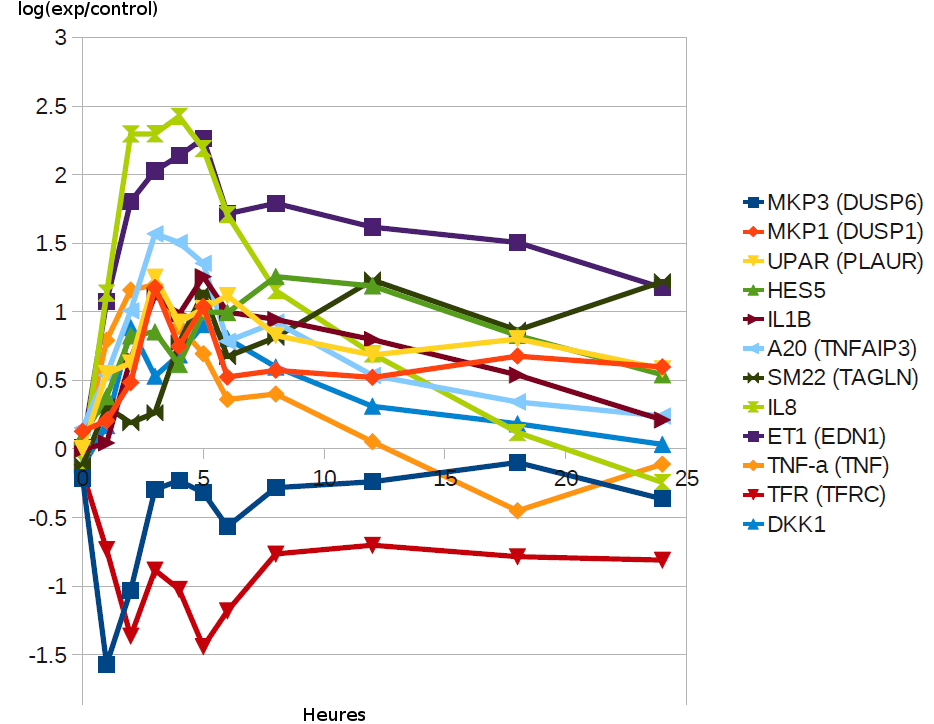
\includegraphics[scale=0.5]{images/12genes.png}
\caption{\label{fig:12genes}
Données de séries temporelles des gènes du réseau.
}
\end{figure}


\section{Process Hitting}\label{sec:PH}
Une façon de modéliser des Réseaux de Régulation Biologiques à l'aide de $\pi$-calcul, appelée Process Hitting (ou Frappes de Processus), a été récemment introduite par l'équipe MeForBio
dans \cite{PMR10-TCSB,PaulevePhD}.
Elle propose un point de vue plus modulable des influences entre composants grâce à une représentation d'actions atomiques entre ceux-ci.
Cette représentation particulière offre des possibilités d'analyse statique efficaces permettant de sur-approximer et sous-approximer l'atteignabilité d'un processus \cite{PMR12-MSCS}.
De plus, son atomicité permet d'adopter différents niveaux d'abstraction dans la modélisation, afin notamment de représenter une sur-approximation du comportement d'un système dont la spécification des coopérations ne serait pas entièrement déterminée.
Une méthode efficace de détermination des points fixes a aussi été développée.
La figure \ref{fig:exPH} donne un exemple de Process Hitting.

Plusieurs extensions ont aussi été proposées pour enrichir ce formalisme.
Une première repose sur l'introduction de la stochasticité afin de modéliser la durée d'évolution relative des composants à l'aide des probabilités.
Cette extension nécessite une simulation de l'exécution du modèle afin d'en extraite des propriétés empiriques, ou l'utilisation d'un model checker.
Une seconde extension consiste en l'attribution de classes de priorités aux actions, afin d'imposer formellement un ordre de tir entre celles-ci.
Cette sémantique reposant sur des priorités fixes permet de modéliser des comportements plus fins, par exemple au niveau des coopérations.
Elle ne modifie pas les résultats concernant la recherche de points fixes.

\begin{figure}[h]
\centering
\scalebox{1.1}{
\begin{tikzpicture}
\path[use as bounding box] (-2,-5.2) rectangle (7,0.7);

\TSort{(0,0)}{b}{2}{t}
\TSort{(0,-3.8)}{c}{2}{b}
\TSort{(4.5,-3)}{a}{3}{r}

\TSetTick{bc}{0}{00}
\TSetTick{bc}{1}{01}
\TSetTick{bc}{2}{10}
\TSetTick{bc}{3}{11}
% \TSetSortLbcel{bc}{$\neg a\wedge b$}
\TSort{(-0.5,-2)}{bc}{4}{b}

\THit{b_1}{bend right}{bc_0}{.north}{bc_2}
\THit{b_1}{bend right}{bc_1}{.north}{bc_3}
\THit{b_0}{}{bc_2}{.north west}{bc_0}
\THit{b_0}{}{bc_3}{.north west}{bc_1}

\THit{c_0}{}{bc_1}{.south}{bc_0}
\THit{c_0}{}{bc_3}{.south}{bc_2}
\THit{c_1}{}{bc_0}{.south}{bc_1}
\THit{c_1}{}{bc_2}{.south}{bc_3}

\path[bounce, bend right=25]
\TBounce{bc_2}{}{bc_0}{.north east}
\TBounce{bc_3}{}{bc_1}{.north east}
;
\path[bounce, bend left=80, distance=30]
\TBounce{bc_0}{}{bc_2}{.north}
\TBounce{bc_1}{}{bc_3}{.north}
;
\path[bounce, bend right]
\TBounce{bc_0}{}{bc_1}{.west}
\TBounce{bc_2}{}{bc_3}{.west}
;
\path[bounce, bend left]
\TBounce{bc_3}{}{bc_2}{.east}
\TBounce{bc_1}{}{bc_0}{.east}
;

\THit{bc_3}{thick}{a_1}{.north west}{a_2}
\THit{bc_0}{thick,bend right=130, in=305, distance=140}{a_1}{.south east}{a_0}
\path[bounce, bend left=40]
\TBounce{a_1}{thick}{a_2}{.south west}
\TBounce{a_1}{thick}{a_0}{.north east}
;

\THit{b_0}{thick,bend left,out=50,in=150}{a_2}{.west}{a_1}
\THit{b_1}{thick,bend left,out=80,in=70,distance=100}{a_0}{.east}{a_1}
\path[bounce]
\TBounce{a_2}{thick,bend right=40}{a_1}{.west}
\TBounce{a_0}{thick,bend right=40}{a_1}{.east}
;

\THit{c_0}{thick,bend left,out=270,in=290, distance=115}{a_2}{.east}{a_1}
\THit{c_1}{thick}{a_0}{.north west}{a_1}
\path[bounce]
\TBounce{a_2}{thick,bend left=40}{a_1}{.north east}
\TBounce{a_0}{thick,bend left=40}{a_1}{.south west}
;

\THit{a_2}{bend left, out=290, in=120}{b_1}{.south}{b_0}
\path[bounce, bend left]
\TBounce{b_1}{}{b_0}{.south}
;

\end{tikzpicture}
}

\caption{\label{fig:exPH}
Exemple de Process Hitting comprenant quatre sortes : $a$, $b$, $c$ et $bc$.
La sorte $bc$ est appelée sorte coopérative (cf. section \ref{sec:PH}).
}
\end{figure}




\chapter{Contributions}

\section{Modélisation}\label{sec:modelisation}
%traduction des patterns des réseaux de signalisations vers le formalisme des frappes de processus

%Ig------->PH
\subsection{Du Graphe d'Interaction(GI) au formalisme des frappes de processus}

Pour traduire notre réseau de signalisation en frappe de processus, nous avons identifié un ensemble de motifs dans le réseau de signalisation auxquels nous avons 
associé les motifs équivalents en frappe de processus. Le tableau \ref{tab:patterns} répertorie quelques exemples de motifs, leurs équivalents en frappes de processus et une brève 
description de leur sémantique. 

En plus de l'identification des motifs, nous avons défini un comportement pour chaque motif. Nous nous sommes inspiré de la sémantique de Thomas\cite{Thomas73}. Ainsi, si un composant est un activateur 
d'un autre composant, il va l'activer s'il est présent et l'inhiber s'il est absent. Réciproquement, si un composant est un inhiteur d'un autre composant, il va l'inhiber s'il est 
présent et le composant s'activera si son inhibiteur est absent. Nous avons en plus des cas simples modélisé les cas les plus complexes comme les décompositions des complexes, les
coopérations entre composants pour influencer la dynamique d'un autre composant et les synchronisations pour également 
influencer la dynamique d'un autre composant.

\begin{table}
\begin{tabular}{|c|c|M{4cm}|}
\hline
\textbf{(A) Les motifs Biologiques}

&

\textbf{(B)équivalents en frappes de processus}

&

\textbf{(C)Brèves descriptions}

\tabularnewline \hline
\begin{tikzpicture}[auto]
\path[use as bounding box] (-0.7,-0.3) rectangle (2.5,2);

\node[qgre] (a) at (0,1) {a};
\node[mod] (i) at (1,1) {i};
\node[qgre] (b) at (2,1) {b};
\node[es] (d) at (1,2) {Simple activation};

\path
 (a) edge[act] (i)
 (i) edge[st]  (b);
\end{tikzpicture}

&


\begin{tikzpicture}
\exphpatact
\end{tikzpicture}

&

Simple activation du composant b par le composant a


\tabularnewline \hline
\begin{tikzpicture}[auto]
\path[use as bounding box] (-0.7,-0.3) rectangle (2.5,2);

\node[qgre] (a) at (0,1) {a};
\node[mod] (i) at (1,1) {i};
\node[qgre] (b) at (2,1) {b};
\node[es] (d) at (1,2) {Simple inhibition};
\path
 (a) edge[inh] (i)
 (i) edge[st]  (b);
\end{tikzpicture}

&

\begin{tikzpicture}
 \exphpatini
\end{tikzpicture}

&

Simple inhibition du composant b par le composant a


\tabularnewline \hline

\begin{tikzpicture}[auto]
\path[use as bounding box] (-0.7,-0.3) rectangle (2.5,3);
\node[qgre] (a) at (0,2) {a};
\node[mod] (i) at (1,1) {i};
\node[qgre] (b) at (0,0) {b};
\node[qgre] (c) at (2,1) {c};
\node[es] (d) at (1,3) {activation or inhibition};

\path
 (a) edge[act] (i)
 (b) edge[inh] (i)
 (i) edge[st]  (c);
\end{tikzpicture}


&

\begin{tikzpicture}
 \exphpatai
\end{tikzpicture}

&

Activation ou inhibition du composant c soit par le composant a soit par le composant b

\tabularnewline \hline

\end{tabular}

\caption{\label{tab:patterns}
Exemples de motifs biologiques (voir colonne (A)) avec les équivalents en frappes de processus (voir colonne (B)) et une brève description de la dynamique sous jacente(voir colonne (C).
}

\end{table}

\subsection{Estimations des paramètres temporels}\label{sec:estimations}
%estimation des paramètres temporelles
La prise en compte de l'aspect temporel et stochastique des réactions biologiques nous contraint à utiliser des paramètres qui 
vont nous permettre d'introduire ces aspects dans notre modèle pour raffiner davantage la dynamique du modèle et permettre de 
mieux capturer la dynamique du système que nous voulons étudier. 

Nous allons nous servir d'un paramètre(le taux) qui va permettre de définir à la fois la durée et la probabilité de survenue d'un évènement.
Le taux d'une action est une approximation de l'inverse  du temps moyen nécessaire pour l'exécution de cette action. L'idée est de faire 
en sorte que le temps moyen nécessaire pour jouer une action, corresponde à l'interval de temps qui sépare cette action de la précédente. Nous 
allons distinguer deux situations: (i) les noeuds ou composants du réseau pour lesquels nous n'avons pas de mesures et (ii) ceux pour lesquels
nous avons les mesures des séries temporelles.

Pour les molécules dont nous n'avons pas de mesures, nous allons choisir le même taux($10$) et le même facteur d'absortion de stochasticité($50$) pour jouer toutes 
les actions.

%Estimation des paramètres temporelles (t1 t2 t3 t4 t5 ...) pour les gènes 
Pour les autres, l'idée de l'estimation des paramètres temporels est de déterminer les différents instants de temps pour lesquels on considère un changement 
d'état à partir des niveaux d'expressions. La détermination des changements d'état va donc s'appuyer sur un choix au préalable des seuils qui 
vont déterminer les différents niveaux d'activités. Ainsi, dès que le niveau d'expression va traverser un seuil, on va considérer qu'il y a un 
changement d'état au niveau du composant. Ce qui doit donc se traduire par une action dans notre modèle qui va entrainer cette dynamique.

Dans un premier temps, nous devons donc déterminer les différents instants $t_{i}$ correspondants à un changement d'état. Par la suite nous devons 
donner les taux aux actions responsables de cette dynamique de façon à pouvoir les observer aux instants estimés.

%intégration des paramètres temporelles sous forme de rate et d'absorption de stochasticité ( r et sa)


%pour les autres molécules



\section{Comparaison des simulations avec les données}

\subsection{Simulation par sous-graphe}

Les premières simulations de notre modèle nous donnent des résultats assez compliqué à analyser. Pour simplifier l'analyse et mieux comprendre
la dynamique de notre modèle, nous nous sommes proposé de l'étudier par sous-graphe. L'idée est de décomposer notre graphe des insteractions en sous-graphes. 
Chaque sous-graphe est un ensemble de composants requis partant d'un gène dont nous voulons observer la dynamique  jusqu'au noeud d'entré du réseau. Nous avons 
ainsi pu analyser  la dynamique de notre réseau par sous-graphe. Nous avons commencé à reconstituer le graphe initial en mettant ensemble les sous-graphes pour
retrouver notre modèle initial(avant décomposition par sous-graphes). Pour terminer 
ce travail nous devons mettre en oeuvre le mécanisme de synchronisation entre les composants dans le formalisme des frappes de processus.


\subsection{Discrétisation des données de séries temporelles}\label{sec:discretisation}
%discretisation des données de séries temporelles
Les données de comparaison sont des données continues et nous voulons les comparer avec les résultats d'un modèle discret. Nous sommes par conséquent 
obligés de discrétiser les données de séries temporelles  pour avoir leur expression discrète afin de pouvoir aisément les comparer avec les résultats 
produits par les simulations de notre modèle.
Nous avons proposé un algorithme de discrétisation qui va prendre en entrée une série temporelle continue et  produire en sortie une série temporelle
discrète sur trois niveaux. L'algorithme \ref{alg:Discretization} détail le principe de la discretisation qui a été utilisé. Nous pouvons observer les résulats 
de la discrétisation en utilisant l'algorithme \ref{alg:Discretization} sur la figure \ref{fig:simulations}.
\begin{algorithm}
\caption{Discretization of experimental data}
\label{alg:Discretization}
\begin{algorithmic}
\REQUIRE $X$ a table of experimental data
\ENSURE $Y$ a table of discretized data
%\STATE $y \leftarrow initialState(x)$
\FORALL{ gene $i$ in $X$ } 

\STATE $threshold \leftarrow computeThreshold(X[i,]);$
\STATE $Y[i,0] \leftarrow initialState(threshold,X[i,]);$
\FORALL {$j$ in $numberExpression$}
  \IF{$Increase(X[i,j],X[i,j+1])$}
   \STATE $computeSignificativityOfIncrease(threshold,X[i,j],X[i,j+1]);$
   \STATE $fixeSTATE(Y[i,j],Y[i,j+1]);$
  \ELSE
   \STATE $computeSignificativityOfDecrease(threshold,X[i,j],X[i,j+1]);$
   \STATE $fixeSTATE(Y[i,j],Y[i,j+1]);$
  \ENDIF
\ENDFOR

\ENDFOR

\end{algorithmic}
\end{algorithm}

%simulations
\subsection{Simulations}\label{sec:simulations}
%préciser qu'il s'agit des sous graphes pour chaque gène

Dans cette section, nous présentons les résultats préliminaire de notre travail. La figure \ref{fig:simulations} nous donne les résultats de la discrétisation et 
de la simulation effectuée sur les sous-graphes de notre modèle pour trois gènes. Nous constatons que nous réussissons à reproduire la dynamique des gènes. De haut en bas,
les trois premier graphiques représentent les tracés des données des séries temporelles continues des trois gènes que nous avons choisi pour illustrer les résultats actuels.
Les trois graphiques suivants représentent les résultats obtenus en effectuant la discrétisation de chaque courbe continue. Enfin les trois derniers graphiques sont les 
courbes obtenues après simulation du modèle. En analysant ces résultats, nous constatons que le modèle permet de reproduire avec certes des imprécisions la dynamique des gènes.
L'aspect stochastique du modèle fait qu'il est difficile d'obtenir avec exactitude la dynamique voulue. Dans la prochaine section nous allons présenter quelques perspectives à ce 
travail.

\begin{figure}[p]
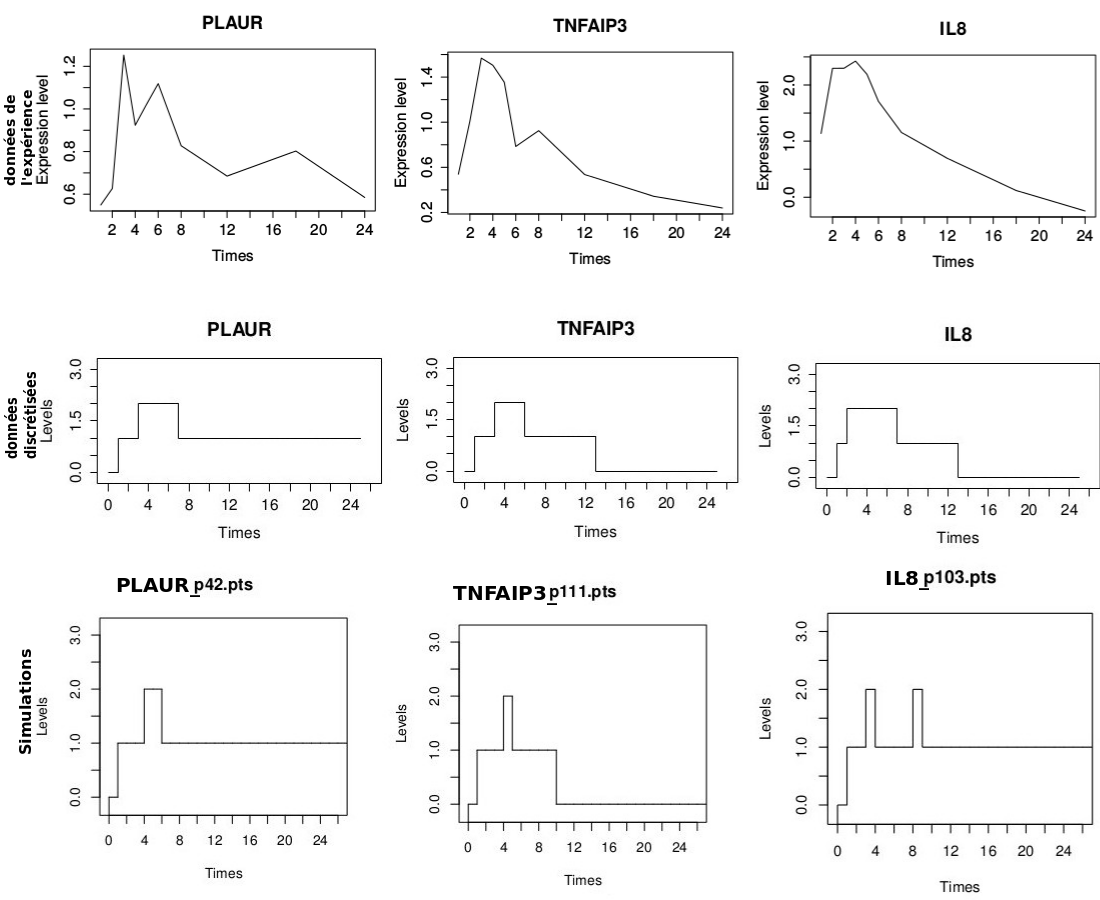
\includegraphics[scale=0.35]{images/courbe-cst1.png}
\caption{\label{fig:simulations}
Résultats de la discrétisation et de la simulation.
}
\end{figure}

\chapter{Perspectives}

A court terme, nous allons proposer des simulations du modèle complet. Pour ce faire nous devons mettre ensemble les sous-graphes pour reconstituer le modèle
complet. Cette reconstitution exige la msie en oeuvre du mécanisme de synchronisation entre les composants qui ont une influence indépendante sur un autre 
composant. En effet, nous avons observé que des composants qui agissent de façon indépendante sur un autre composant peuvent générer des oscillations. Ce comportement
n'est pas cohérent avec la dynamique que voulons générer. Pour cette réaison nous avons décidé de mettre en oeuvre le mécanisme de synchronisation dans le formalisme 
des frappes de processus. En plus de cette perspective immédiate, nous allons présenter dans la suite les autres perspectives de ce travail.

\section{Notion de reconnaissance automatique  de trace}\label{sec:trace}
On peut comparer deux systèmes de transitions pour voir leur évolution au fur et à mesure que les transistions sont tirées. L'évolution d'un système peut être 
représentée par la trace du chemin issu de l'état initial ou un autre. On peut alors analyser les traces et voir comment un système se comporte par rapport à un autre.
En particulier, on peut chercher à savoir si des traces sont identiques, si l'une est incluse dans l'autre, si les deux traces ont les sous-traces communes spécifiques.
Nous comptons sur la base de cette idée mettre en oeuvre un mécansme de reconnaissance automatique des traces qui seront générées après simulation du modèle. L'objectif est
de pouvoir comparer de façon automatique un résultat d'une simulation avec une courbe discrete sur la base des critères objectifs.


\section{Etude stochastique}\label{sec:verification}

Le modèle que nous avons construis est un modèle qui prend en compte l'aspect stochastique des systèmes biologiques. Nous nous proposons d'effectuer une étude stochastique de 
ce modèle afin de pouvoir mettre en évidence un ensemble de propriétés liées à l'aspect stochastique du focntionnement du modèle. Un des objectifs majeur de cette perspective est 
de pouvoir faire des prédictions stochastiques des dynamiques que nous pourrions observer en fonction du nombre de simulation et des paramètres stochastiques du modèle. Nous 
espérons aussi pouvoir mettre en évidence un ensemble de caractéristiques stochastiques qui vont nous permettre d'influencer la dynamique du modèle.

\section{Vérification logique et Processus Clés} \label{sec:keyplayer}
Outre l'étude stochastique du modèle, nous allons nous intéresser à une vérification logique des propriétés du modèle afin de proposer les éléments pour le contrôle de 
la dynamique du réseau. Nous comptons nous intéresser à la détection des processus clés. Ici un processus clé est un processus tel que son activité(actif ou inactif) modifie la dynamique du réseau ou 
d'une sous partie du réseau.

\section{Mise en oeuvre sur un cas réel biologique}\label{sec:miseenoeuvre}
Les résultats concernants l'analyse dynamique du système et les processus clés seront validés expérimentalement par des analyses fonctionnelles
des gènes clés du système de différentiation cellulaire via l'interférence basée sur shRNA dans les kératinocytes humains primaires.


\chapter{Autres activités}

\section{Production scientifique}

\textbf{Article court soumis et accepté avec présentation d'un exposé oral}\\
Louis Fippo Fitime, Andrea Beica, Olivier Roux and Carito Guziolowski:
\textbf{Integrating time-series data on large-scale cell-based models: application to skin differentiation}.
Proceedings of the Evry Spring School, pages 57-72. 2014.

\section{Ecoles et Formations suivies}

\begin{itemize}
\item \textbf{AVANCÉES EN BIOLOGIE DES SYSTÈMES ET DE SYNTHÈSE (ASSB'14)},
Modélisation de systèmes biologiques complexes dans le contexte de la génomique.\\
École Thématique de Recherche\\
Du 24 au 28 mars 2014, Évry, France 

\item \textbf{École d'été sur la Modélisation et Vérification des Systèmes Parallèles (MOVEP'14)},\\
7-11 juillet 2014, Nantes, France 

\item \textbf{Formation doctorale : Estimation des incertitudes}\\
Type formation Cours \\
Durée: 15:00 heures
\end{itemize}

\section{Enseignements}

%\bigskip

\noindent
\textbf{Méthodes logicielles (MELOG) :} 2\textsuperscript{e} année (semestre 6)\\
Programmation orientée objet, structures de données et langage Java\\
\textbf{Responsable :} Guillaume MOREAU
\begin{itemize}
  \item 2 groupes de TP, soit 28 heures
\end{itemize}

\noindent
\textbf{Algorithmique et programmation (ALGPR) :} 1\textsuperscript{ère} année (semestre 6 et 7)\\
Introduction à l'algorithmique et applications au langage C\\
\textbf{Responsable :} Vincent TOURRE
\begin{itemize}
  \item 2 groupes de TP, soit 40 heures
\end{itemize}

\section{Activités collectives}
Membre du bureau en tant que vice-trésorier et correspondant IRCCyN des membres de l'\emph{Association des Étudiants en Doctorat de l'École Centrale de Nantes} (AED).


\bibliographystyle{alpha}
\bibliography{biblio}


\end{document}
